\documentclass[a4paper,10pt]{report}
\usepackage[utf8x]{inputenc}
\usepackage{graphicx}
\usepackage[brazil]{babel}
\usepackage{hyperref}
\usepackage{html,makeidx}

%specific to HTML output
%\htmltitle{Fundamentos de Computação Gráfica - INF2608}
%\htmladdress{robertogerson@telemidia.puc-rio.br}
%\htmlcss{http://www.w3.org/StyleSheets/Core/Modernist}

% Title Page
\title{Fundamentos de Computação Gráfica - INF2608}
\author{Roberto Gerson de Albuquerque Azevedo}

\begin{document}
\maketitle

\begin{abstract}
Este documento apresenta a base teórica para os trabalhos desenvolvidos no
escopo da disciplina \htmladdnormallink{Fundamentos
de Computação Gráfica (FCG) -
INF2608}{http://www.tecgraf.puc-rio.br/~mgattass/fcg/fcg.html}, cursada
durante o Doutorado em Informática pela PUC-Rio. A disciplina de FCG é subdivida
em três partes principais: Luz e Cor, Imagem e 3D. Para cada uma dessas partes é
sugerido o desenvolvimento de um projeto. As seções a seguir detalham cada um
desses projetos.
\end{abstract}

\chapter{Luz e Cor}
\par
Sendo a Computação Gráfica (CG) a área da computação destinada ao estudo de
modelos e algoritmos para o processamento de imagens digitais, o estudo da cor é
um dos seus fundamentos. A cor é uma sensação humana que os seres humanos têm
em resposta à luz incidente em nossos olhos. Sendo assim, o estudo da cor está
diretamente relacionado com o estudo da luz.

\par


\section{Enunciado do Trabalho}
\par
Um dos padrões de cor mais difundidos é o \textit{Macbeth Color Checker}
ilustrado na figura abaixo.

\begin{figure}[!htb]
     \centering
     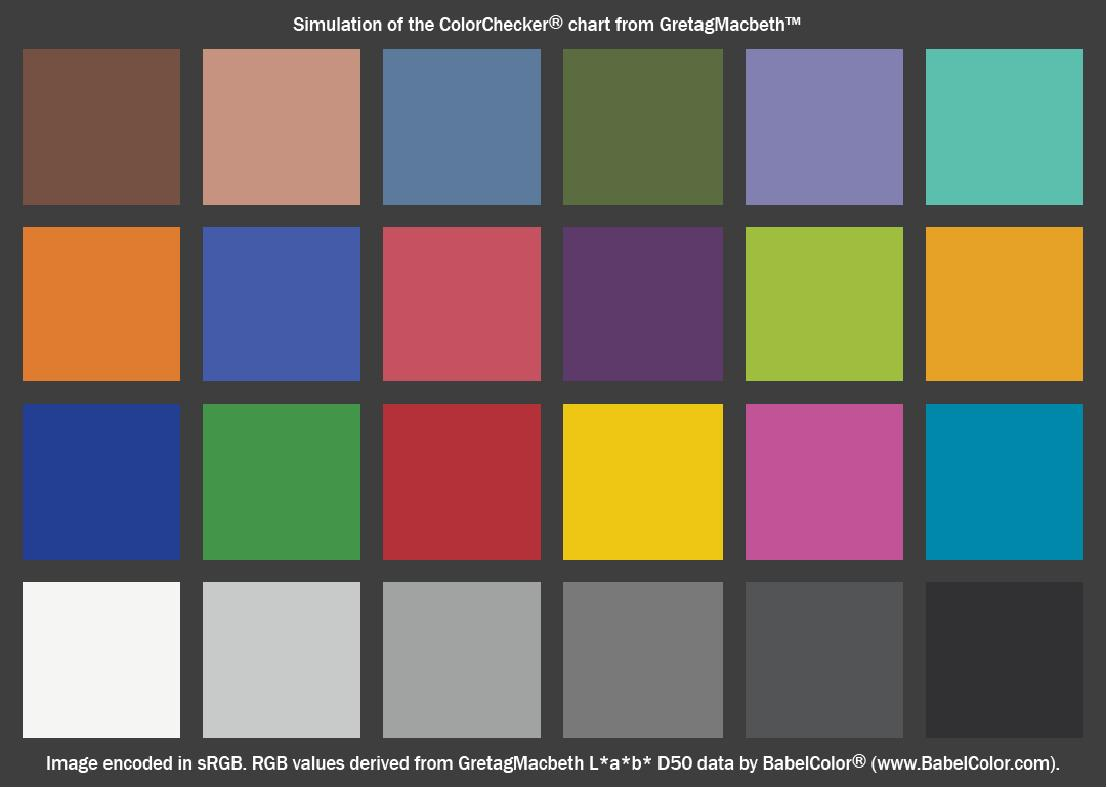
\includegraphics[scale=0.4]{img/colorChecker.jpg}
     \caption{Macbeth Color Checker. Fonte: URL}
     \label{Label de referência para a imagem}
\end{figure}

\par
Considere as amostras armazenadas por linha da esquerda para a direita de cima
para baixo.  Desta foram na última linha temos os tons de cinza e as quatro
primeiras cores são: pele escura(dark skin), pele clara(light skin), azul céu
(blue sky) e folhagem (foliage), respectivamente.  

\par
O trabalho de cor deste ano consiste em:
\newcounter{qcounter}
\begin{list}{\arabic{qcounter}:~}{\usecounter{qcounter}}
\item A partir do espectro fornecido calcular as componentes CIEXYZ,
CIExyY, CIELuv, CIELab e sRGB destas quatro primeiras amostras.
\item Somar os espectros da pele clara com o céu azul e calcular, a partir deste
novo espectro as componentes CIEXYZ, CIExyY, CIELuv, CIELab e sRGB.
\item Verificar a linearidade destes sistemas.
\end{list}

\section{Percepção da Cor}
\subsection{Observador padrão CIE}
\par


\subsection{Adaptação do sistema humano}
\par
Adaptação da visão (luz/escuro)

\par
Influência do ambiente (tamanho, cor de background etc.). Transformar a
cor de um display para que tenha a mesma aparência impressa. Outro exemplo:
dado a cor em um background, calcular a cor que "aparenta ser a mesma" e

\par
Modelos da aparência de cor. Um modelo de aparência de cor deve considerar
todas as cores em uma imagem, ao invés da cor dos pixels individualmente.

\par
Medida dos Estimulus Físicos -> Cálculo dos Três estímulos -> Cálculo dos
atributos perceptuais.

\section{Espaços de Cor}

\subsection{CIEXYZ}
Soon.

\subsection{CIExyZ}
Soon.

\subsection{CIELuv}
Soon.

\subsection{CIELab}
Soon.

\subsection{RGB}
Soon.

\subsection{sRGB}
Soon.

\section{Implementação}
Soon.

\section{Linearidade dos Espaços de Cor}
Soon.

\section{Arquivos}
Soon.

\section{Instalação a partir do código-fonte}
This repository is for Roberto Azevedo's programs developed in the scope of the
Foundations of Computer Graphics discipline. This discipline was coursed during
the Roberto Doctoral course in Pontificial Catholic University of Rio de Janeiro
(PUC-Rio). Marcelo Gattass (http://www.tecgraf.puc-rio.br/~mgattass) was the
teacher.

Computer Graphics, PUC-Rio, Color, Image, 3D

\chapter{Imagem}
Soon.

\chapter{3D}
Soon.

\end{document}
